\chapter{Materiais e métodos}

Este projeto adota um delineamento observacional, prospectivo e analítico, com o objetivo de validar algoritmos de rPPG para extração de sinais fisiológicos em pacientes críticos internados na UTI do Hospital Universitário da Universidade de São Paulo. O estudo foi aprovado pelo Comitê de Ética em Pesquisa da instituição sob o número Certificado de Apresentação de Apreciação Ética (CAAE) 86650625.3.0000.0076. Todos os dados são coletados com permissão explícita dos indivíduos envolvidos ou de seus representantes. 

\section{Aquisição de dados}

A aquisição de dados é realizada por meio da gravação de vídeos da face de pacientes internados na UTI realizada com uma câmera industrial sob condições de iluminação ambiente do leito e sem imposição de nenhuma restrição ao indivíduo monitorado. Cada gravação tem duração aproximada de dois minutos e a câmera é posicionada ao pé da cama hospitalar, conforme demonstra a Figura \ref{fig:setupcoleta}, caso o paciente esteja deitado, ou a uma distância fixa próxima de 180 centímetros, caso o paciente esteja sentado na poltrona também disponível no local de internação. Ademais, são coletados dados sobre a iluminação medida na região próxima ao rosto, com o uso de um luxímetro digital de modelo Fluke 941 e é realizada a medição do fototipo de acordo com a escala Fitzpatrick com um Analisador de Fototipo de Pele Digital da \textit{Skinup Beauty Devices} posicionado na testa. Simultaneamente, são extraídos dados fisiológicos de referência do sinal do eletrocardiograma com taxa de amostragem de 250 Hz, da frequência respiratória com taxa de amostragem de 125 Hz e da onda de fotopletismografia obtida por meio de um oxímetro de pulso com taxa de amostragem de 62,5 Hz. Todos os sinais fisiológicos são adquiridos diretamente dos monitores multiparâmetros de modelo BSM-3000 Series da Nihon Kohden já instalados à beira-leito, utilizando um sistema de coleta previamente implementado para comunicação com os dispositivos.

\begin{figure}[h]
    \centering
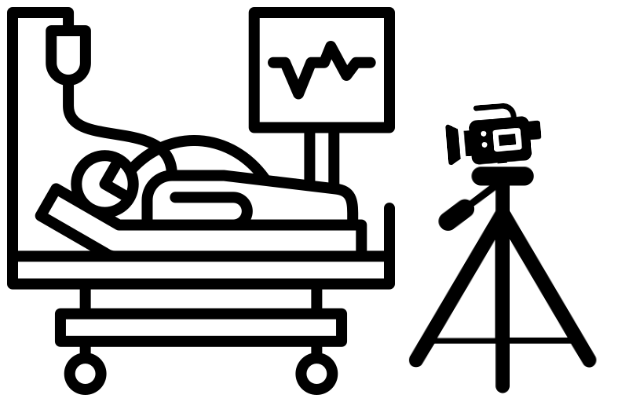
\includegraphics[width=0.5\linewidth]{imagens/setup_coleta.png}
    \caption{Esquemático do ambiente de coleta de dados} 
    Fonte: autoria própria
    \label{fig:setupcoleta}
\end{figure}

A aquisição de dados foi estruturada em três procedimentos diferentes, sendo eles:

\begin{enumerate}
    \item \textbf{Coleta preliminar}

    Foi realizada uma coleta preliminar de dados de três pacientes internados na UTI, com uma câmera do modelo VCXG.2-57C da Baumer configurada com taxa de 25 quadros por segundo, formato de pixel BR8. Para cada paciente, o tempo de exposição, ganho, foco e abertura do sensor foram definidos de forma a garantir a máxima visualização com o mínimo de sombras e sem saturação de pixels. A resolução, por sua vez, foi definida de forma a enquadrar o rosto e parte do tórax e os vídeos são capturados em formato AVI. Além disso, a distância entre cada indivíduo e a câmera variou de acordo com a disposição do paciente dentro do ambiente de internação, sendo que esse valor variou entre 170 e 190 centímetros, já que dois dos pacientes estavam deitados na cama reclinada e um dos pacientes estava sentado em uma poltrona ao lado da cama.  

    \item \textbf{Coleta de validação}

    Em um segundo momento, foi realizada a coleta de três vídeos em formato AVI de 2 minutos e 5 segundos de duração de um indivíduo saudável não hospitalizado com uma câmera do modelo VCXU.2-57C com 50 quadros por segundo, com uma resolução fixa de 1056x1076 e tempo de exposição fixo em 19500 milissegundos. O ganho, foco e abertura do sensor foram definidos de forma a garantir a máxima visualização com o mínimo de sombras e sem saturação de pixels. Além disso, a distância entre o indivíduo e a câmera foi definida como 140 centímetros. Nesse caso, foi adquirido o sinal de eletrocardiograma com um equipamento de eletromiografia e registro de potenciais evocados do modelo MEB-2300K da Nihon Kohden com frequência de amostragem de 1000 Hz e eletrodos posicionados no dorso das mãos e nos tornozelos para a medição da derivação DII. No início de cada gravação, foi gerado um ruído em um eletrodo de ECG visível no enquadramento para sincronização posterior entre os quadros capturados e o sinal de referência, conforme será elaborado adiante. Esse procedimento foi executado com o intuito de validar a aplicação dos algoritmos considerados, os quais serão expostos em diante, em um indivíduo saudável.

    \item \textbf{Coleta definitiva}

    Para a coleta definitiva, serão adquiridos vídeos de 2 minutos e 5 segundos de duração de ao menos 10 pacientes com a câmera de modelo VCXU.2-57C com 50 quadros por segundo, sob os mesmos procedimentos de ajuste do sensor óptico que os adotados na coleta de validação. Nesse caso, a distância entre a câmera e o paciente é condicionada pela disposição da instalação e pelo posicionamento do indivíduo dentro dela. Ademais, os dados de referência serão coletados dos monitores multiparâmetros, da mesma maneira descrita para a coleta preliminar.

\end{enumerate}

A diferença da câmera em cada procedimento se dá devido à disponibilidade, dado que a coleta preliminar foi realizada com uma câmera provisória disponibilizada pela empresa fabricante, enquanto as outras coletas dependem da aquisição definitiva do segundo modelo. Ademais, a escolha da utilização de uma câmera industrial é baseada sobretudo no objetivo de garantir a aquisição de dados sem compressão, já que esse é um fator que deteriora significativamente a relação sinal-ruído, conforme discutido na \autoref{sec:influencing-factors}. Além disso, a obtenção de imagens de boa qualidade em um sistema cujos parâmetros do sensor óptico podem ser configurados de forma acessível garante a robustez na análise dos algoritmos. 

\subsection{Sincronização de dados}

A aquisição dos dados de vídeo é realizada com a duração de aproximadamente 2 minutos, ao passo que os dados de referência, em todos os procedimentos de coleta, são gravados em um intervalo de tempo maior que o do vídeo e que abrange o momento de sua gravação. Assim, é necessária a sincronização desses sinais para o posterior processamento e análise. Isso é realizado com base na comparação entre o horário de aquisição dos vídeos e os registros temporais referentes aos sinais fisiológicos. Como esses horário não são necessariamente coincidentes, apesar de sempre serem próximos, são necessárias etapas específicas a cada procedimento de coleta de dados. 

\begin{itemize}
    \item \textbf{Coleta preliminar}

    O único protocolo de sincronização de dados nesse procedimento de coleta foi o registro dos horários de início e fim da gravação do vídeo e do horário apresentado no monitor multiparâmetros no instante do início da gravação. Desse modo, como os dados de referência são capturados de forma contínua, a sincronização dos dados de uma captura de vídeo específica baseia-se na obtenção do intervalo de tempo dentro dos registros temporais dos sinais de referência na qual foi realizada essa captura. Para isso, é aplicada uma análise de correlação entre os valores de frequência cardíaca estimados a partir dos sinais obtidos remotamente e os valores de referência extraídos do ECG em um intervalo suficientemente grande. 
    
    Dessa maneira, assume-se que a diferença entre os relógios do sistema de armazenamento dos dados dos monitores e do computador responsável por registrar os vídeos não excede três minutos. Dessa forma, define-se uma janela temporal de oito minutos que engloba o horário indicado pelo monitor no momento da aquisição. A partir dessa janela, são extraídos os dados brutos do ECG e a frequência cardíaca é estimada utilizando a biblioteca HeartPy \cite{heartpy}, com janelas deslizantes de 15 segundos e passo de um segundo. Em paralelo, os sinais de BVP são obtidos a partir dos vídeos por meio de 7 métodos não supervisionados de rPPG, os quais serão expostos adiante, sendo que os vídeos foram subdivididos em janelas de 15 segundos. Para cada janela, a frequência cardíaca é estimada no domínio da frequência por meio da FFT, considerando o pico espectral do sinal previamente filtrado na faixa de 0,6 a 3,3 Hz. Por fim, para cada método de rPPG, as séries temporais de frequência cardíaca obtidas remotamente e as séries obtidas a partir do ECG são alinhadas por meio de uma análise de correlação cruzada baseada no índice de correçação de Pearson, na qual a série derivada da rPPG é transladada temporalmente em relação à série de referência do ECG, com passo de um segundo, conforme é explicitado na Figura \ref{fig:sinc-L9} do \autoref{cap:results}. Desse modo, o intervalo de dois minutos, que é o tempo de duração de cada vídeo, que apresenta o maior coeficiente de correlação médio é selecionado para a extração final dos dados de referência.

    \item \textbf{Coleta de validação}

    Nessa coleta, em cada gravação, foi gerado um ruído em um dos eletrodos de eletrocardiograma do indivíduo monitorado de forma visível no enquadramento da imagem da câmera. Assim, o primeiro quadro do vídeo em que é identificada a interferência no eletrodo é utilizado de forma que os quadros anteriores são desconsiderados. Além disso, o vídeo é cortado de modo que são consideradas as imagens capturadas 5 segundos após esse quadro para a extração do sinal sem a interferência desse artefato. Ademais, o ruído gerado, causado por um impacto no eletrodo, gera um pico distinguível na forma de onda do sinal de ECG, de forma que o intervalo considerado para o sinal de referência possui início no instante 5 segundos após o momento respectivo a esse pico e tem duração igual à do vídeo correspondente já editado. 

    \item \textbf{Coleta definitiva}

    Nessa coleta, serão realizados os mesmos procedimentos de sincronização de dados adotados na coleta de validação.
    
\end{itemize}

\section{Processamento de dados de vídeo}

Os dados de vídeo são processados com o uso do conjunto de ferramentas de código aberto denominado rPPG-Toolbox \cite{liu2022rppg}, o qual disponibiliza implementações dos principais métodos não supervisionados de extração de sinais por fotopletismografia remota. Além disso, esse recurso inclui modelos supervisionados para treinamento e teste em bases de dados de acesso livre, além de permitir a inclusão de modelos e bases customizados. Com isso, propõe-se a validação dos algoritmos mostrados na \autoref{tab:metodos_rppg} nos dados coletados dos pacientes de UTI, por meio da inserção de um dataset customizado e da adaptação do conjunto de ferramentas citado.

\begin{table}[ht]
\centering
\caption{Métodos a serem validados nos dados coletados de pacientes de UTI}
\label{tab:metodos_rppg}
\begin{tabular}{|c|l|p{5cm}|}
\hline
\textbf{Tipo} & \textbf{Método} & \textbf{Estratégia} \\ \hline

\multirow{12}{*}{Não supervisionado}
& GREEN \cite{verkruysse2008remote} & Análise do canal verde\\ \cline{2-3}
& ICA \cite{poh2010advancements} & Separação cega de sinais \\ \cline{2-3}
& CHROM \cite{de2013robust} & Modelo baseado em crominância \\ \cline{2-3}
& PBV \cite{de2014improved} & Modelo do vetor de pulso \\ \cline{2-3}
& POS \cite{wang2016algorithmic} & Projeção no subespaço ortogonal ao tom de pele\\ \cline{2-3}
& LGI \cite{pilz2018local} & Modelagem de variações espaciais para robustez a movimento \\ \cline{2-3}
& OMIT \cite{casado2023face2ppg} & Modelagem baseada em decomposição de matrizes \\ \hline

\multirow{7}{*}{Supervisionado}
& DeepPhys \cite{chen2018deepphys} & CNN 2D com mecanismo de atenção \\ \cline{2-3}
& TSCAN \cite{liu2020multi} & CNN 2D com módulos de deslocamento temporal \\ \cline{2-3}
& PhysNet \cite{yu2019physnet} & CNN 3D \\ \cline{2-3}
& PhysFormer \cite{yu2022physformer} & Transformer Visual \\ \cline{2-3}
& EfficientPhys \cite{liu2023efficientphys} & Swin Transformer\\ \hline

\end{tabular}
\end{table}

Para isso, em cada vídeo de entrada, é realizada a detecção da face utilizando a ferramenta YOLO5Face \cite{qi2022yolo5face} a cada 25 quadros, sendo que a região de interesse selecionada é a região retangular retornada por essa ferramenta. Em seguida, os quadros recortados nessa região são utilizados como entrada para os algoritmos de rPPG. No caso especificamente dos algoritmos não supervisionados, é realizada, ainda, a média espacial dos pixels de cada quadro para o processamento das variações das intensidades dos canais de cor. Em relação à validação dos métodos baseados em aprendizado profundo, serão considerados os modelos treinados no dataset denominado PURE \cite{stricker2014pure} e no dataset referido como UBFC-rPPG \cite{bobbia2019unsupervised}.

A partir da onda de pulso resultante dos algoritmos considerados, a frequência cardíaca é estimada por análise em frequência utilizando a FFT em janelas subsequentes de 15 segundos, sendo que o pico do espectro de potência do sinal filtrado por um filtro passa-banda entre as bandas de 0,6 e 3,3 Hz é considerado como a frequência cardíaca. Ademais, a frequência respiratória pode ser estimada por três métodos de análise das modulações do sinal de rPPG causadas pela respiração, sendo eles a análise da modulação de linha de base (BW), a análise da modulação de amplitude (AM) e a análise da modulação de frequência (FM). Para isso, o sinal inicial extraído com um dos algoritmos de rPPG definidos é filtrado por um filtro passa-altas na banda referente a 4 respirações por minuto. Cada um dos métodos é aplicado em cada ponto do ciclo da onda de pulso extraída remotamente para obter a respectiva sequência discreta de amostras correspondente ao tipo de modulação em questão. 

A análise da modulação de linha de base baseia-se na média entre as amplitudes de um ponto de vale e do pico subsequente, conforme a equação:

\begin{equation}
    \label{eq:B}
    BW(n) = \frac{A_{vale}(n) + A_{pico}(n)}{2}
\end{equation}

em que \(A_{vale}(n)\) é a amplitude do vale de um ponto \(n\) da onda de rPPG e \(A_{pico}(n)\) é a amplitude do pico subsequente a esse ponto. A implementação desse cálculo em todos os ciclos do sinal permite extrair a sequência discreta de amostras \(BW\) da linha de base do sinal de rPPG, conforme mostra a \autoref{fig:bw}.

\begin{figure}[h!]
    \centering
    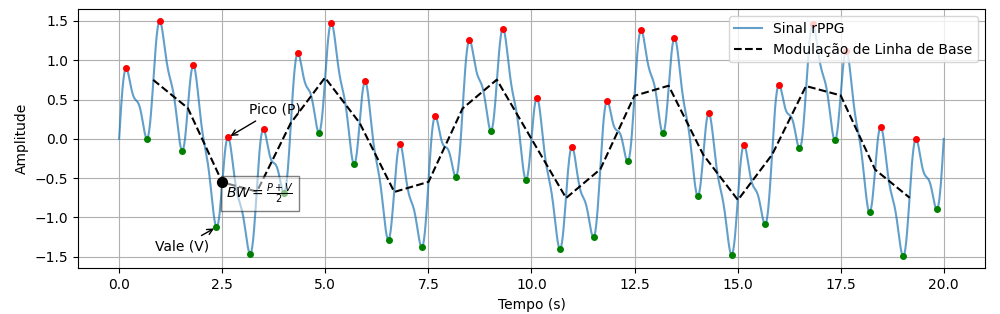
\includegraphics[width=0.9\linewidth]{imagens/bw.png}
    \caption{Extração da modulação de linha de base no sinal de rPPG causada pela respiração}
    Fonte: autoria própria
    \label{fig:bw}
\end{figure}

A análise da modulação de amplitude do sinal de rPPG causada pela respiração é baseada na diferença entre as amplitudes de um ponto de vale e do pico subsequente, conforme a equação:

\begin{equation}
    \label{eq:am}
    AM(n) = A_{pico}(n) - A_{vale}(n)
\end{equation}

em que \(AM\) é a sequência discreta de amostras da modulação de amplitude do sinal de rPPG, como exemplifica a \autoref{fig:am}.

\begin{figure}[h!]
    \centering
    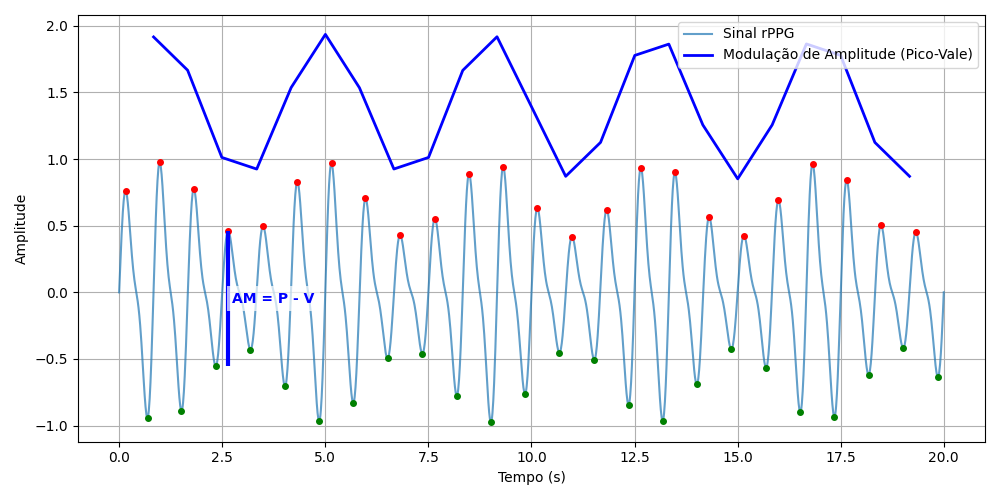
\includegraphics[width=0.9\linewidth]{imagens/am.png}
    \caption{Extração da modulação de amplitude do sinal de rPPG causada pela respiração}
    Fonte: autoria própria
    \label{fig:am}
\end{figure}

A análise da modulação de frequência no sinal de rPPG causada pelos fenômenos respiratórios, por sua vez, é realizada  considerando o intervalo entre picos consecutivos, de acordo com a equação:

\begin{equation}
    \label{eq:fm}
    FM(n) = t(n) - t(n-1)
\end{equation}

em que \(t(n)\) é o instante referente ao pico \(n\) e \(t(n-1)\) é o instante referente ao pico anterior. A implementação desse cálculo em todos os ciclos do sinal permite extrair a sequência discreta de amostras \(FM\) dos intervalos entre picos do sinal de rPPG, conforme mostra a \autoref{fig:fm}.

\begin{figure}[h!]
    \centering
    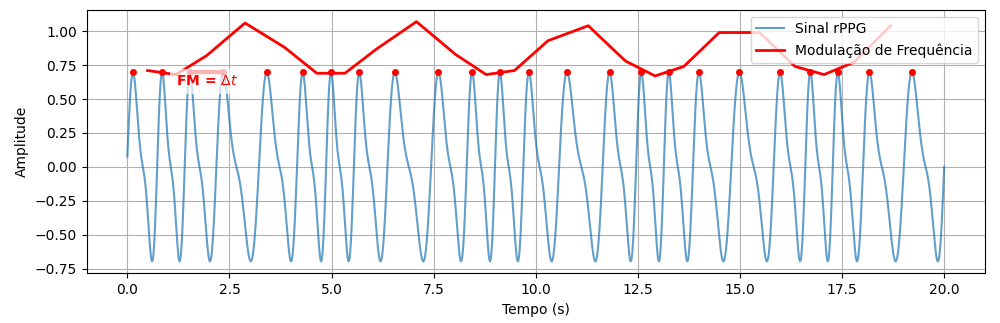
\includegraphics[width=0.9\linewidth]{imagens/fm.png}
    \caption{Extração da modulação de frequência do sinal de rPPG causada pela respiração}
    Fonte: autoria própria
    \label{fig:fm}
\end{figure}

Assim, as sequências discretas referentes às modulações de amplitude e de linha de base são re-amostradas em uma grade temporal uniforme de 4 Hz por meio de interpolação linear. Já a sequência referente à modulação de frequência é re-amostrada em uma grade temporal uniforme de 4 Hz por meio do algoritmo de Berger \cite{berger1986efficient}, uma vez que é derivada de intervalos entre picos do sinal de pulso obtido remotamente e não representa uma amostragem pontual do sinal no tempo. A partir disso, a frequência respiratória é estimada a partir de cada uma das sequências interpoladas por meio de análise espectral, de forma que a frequência com maior energia no espectro de potência obtido por FFT dentro das bandas esperadas nesse contexto, de 4 a 65 respirações por minuto, é considerada como o valor de frequência respiratória obtido pelo método correspondente. Esse processo é realizado em janelas subsequentes de 30 segundos do sinal de rPPG original. Em seguida, a fim de reduzir interferências de artefatos de ruído, é realizada uma estratégia de fusão das estimativas de frequência respiratória realizadas pelos 3 métodos, de modo que a estimativa final é uma média desses 3 valores. No entanto, de maneira a garantir a robustez dessa estratégia, esse valor só é considerado confiável caso o desvio padrão entre as estimativas seja menor que 4 respirações por minuto \cite{charlton2016assessment, luguern2020assessment}.

\section{Processamento dos dados de referência}

Paralelamente, para a construção da base de dados proposta, são utilizados os dados de referência coletados dos monitores multiparâmetros e devidamente sincronizados com os vídeos. Para tanto, é extraído o sinal do eletrocardiograma considerado como padrão-ouro para a obtenção da frequência cardíaca, sendo que esse parâmetro é calculado utilizando a biblioteca HeartPy \cite{heartpy}, com janelas de 15 segundos. A forma de onda fotopletismográfica, por sua vez, obtida com um oxímetro de pulso posicionado no dedo indicador, é utilizada para comparação com o sinal de pulso resultante dos algoritmos por meio de uma análise por correlação cruzada. Por fim, o sinal de impedância torácica captado pelos eletrodos de ECG também é extraído como referência para extração da frequência respiratória realizada utilizando a FFT em janelas subsequentes de 30 segundos. Exemplos desses sinais são apresentados na \autoref{fig:sinais-referencia}.

\begin{figure}[h!]
    \centering

    % Linha superior
    \begin{subfigure}{0.45\textwidth}
        \centering
        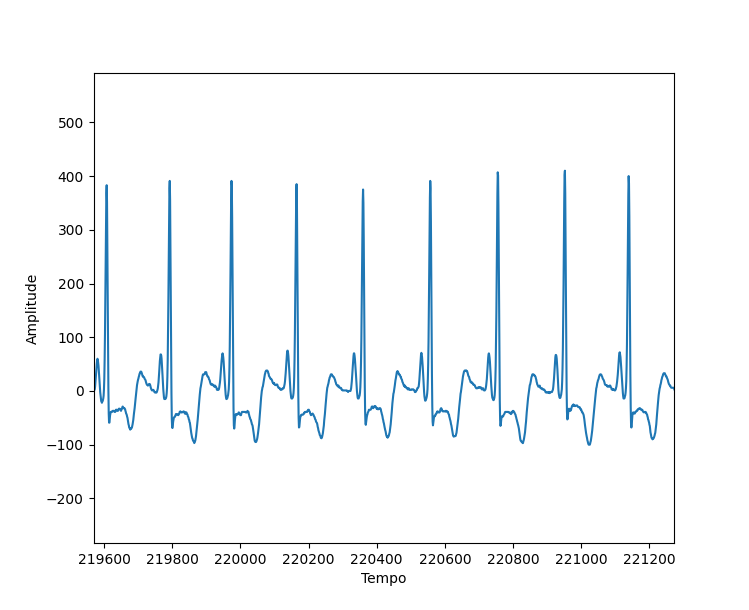
\includegraphics[width=\linewidth]{imagens/ecg_exemplo.png}
        \caption{ECG}
    \end{subfigure}
    \hfill
    \begin{subfigure}{0.45\textwidth}
        \centering
        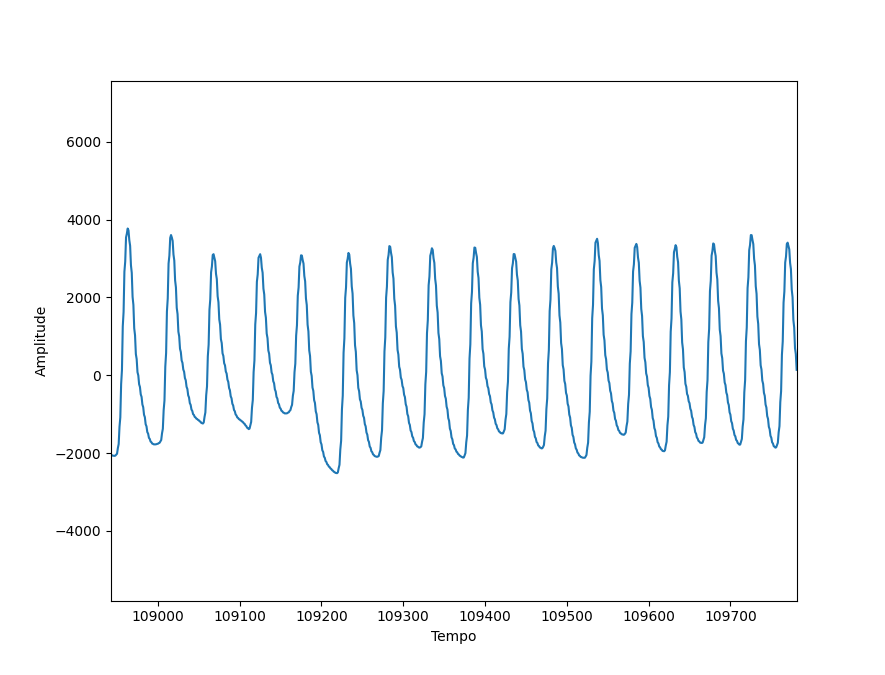
\includegraphics[width=\linewidth]{imagens/PPG_oximetro_exemplo.png}
        \caption{PPG}
    \end{subfigure}

    % Linha inferior
    \begin{subfigure}{0.6\textwidth}
        \centering
        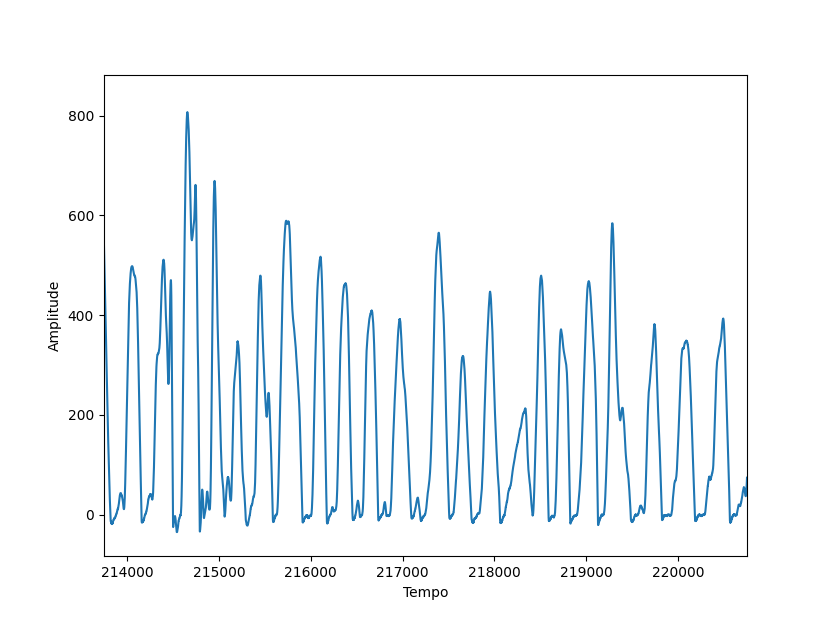
\includegraphics[width=\linewidth]{imagens/impedancia_toracica_exemplo.png}
        \caption{Impedância torácica}
    \end{subfigure}

    \caption{Exemplos de sinais de referência}
    \label{fig:sinais-referencia}
\end{figure}

\section{Métricas de avaliação}

Os parâmetros de frequência cardíaca e frequência respiratória são extraídos em janelas subsequentes do sinal de pulso obtido remotamente, assim como os valores de referência. Assim, são calculadas métricas de comparação entre as janelas coincidentes de cada sinal a fim de quantificar o desempenho de cada algoritmo na estimativa dos parâmetros considerados, de forma que os valores de frequência cardíaca estimados a partir do sinal de rPPG são comparados janela a janela com os valores estimados a partir do ECG. Os valores de frequência respiratória estimados a partir do sinal obtido remotamente, por sua vez, são comparados janela a janela com os valores estimados a partir do sinal de impedância torácica de referência. Nesse sentido, é definido a seguir o cálculo de cada métrica aplicada.

\textbf{Erro Absoluto Médio (MAE)} 
\begin{equation}
    MAE = \frac{1}{N} \sum_{n=1}^{N} \left| R_g - R_p \right|
\end{equation}

\textbf{Erro Quadrático Médio (RMSE)}
\begin{equation}
    RMSE = \sqrt{\frac{1}{N} \sum_{n=1}^{N} (R_g - R_p)^2}
\end{equation}

\textbf{Erro Percentual Absoluto Médio (MAPE)}
\begin{equation}
MAPE = \frac{1}{N} \sum_{n=1}^{N} \left| \frac{R_g - R_p}{R_g} \right|
\end{equation}

\textbf{Índice de Correlação de Pearson (\(\rho\))}
\begin{equation}
\rho = 
\frac{
\sum_{n=1}^{N} (R_{g,n} - \bar{R}_g)(R_{p,n} - \bar{R}_p)
}{
\sqrt{
\left( \sum_{n=1}^{N} (R_{g,n} - \bar{R}_g)^2 \right)
\left( \sum_{n=1}^{N} (R_{p,n} - \bar{R}_p)^2 \right)
}
}
\end{equation}

Em todas as equações, \(R_g\) é o valor de referência, \(R_p\) é o valor estimado por meio do sinal obtido remotamente, \(N\) é o número de amostras de janelas de 15 segundos considerado e \(\bar{R_g}\) e \(R_p\) são as médias desses valores ao longo das amostras. 

\textbf{Relação Sinal-Ruído (SNR)}
\begin{equation}
SNR = 10 \log_{10} \left(
\frac{
\sum_{f=45}^{150} \left( U_t(f) S(f) \right)^2
}{
\sum_{f=45}^{150} \left( (1 - U_t(f)) S(f) \right)^2
}
\right)
\end{equation}
Nesse caso, \(S\) é o espectro de frequência do sinal de rPPG, \(U_t(f)\) é uma função definida como 1 na frequência fundamental e no primeiro harmônico do sinal de referência e como 0 em todos os outros pontos.

\begin{figure}[h]
    \centering
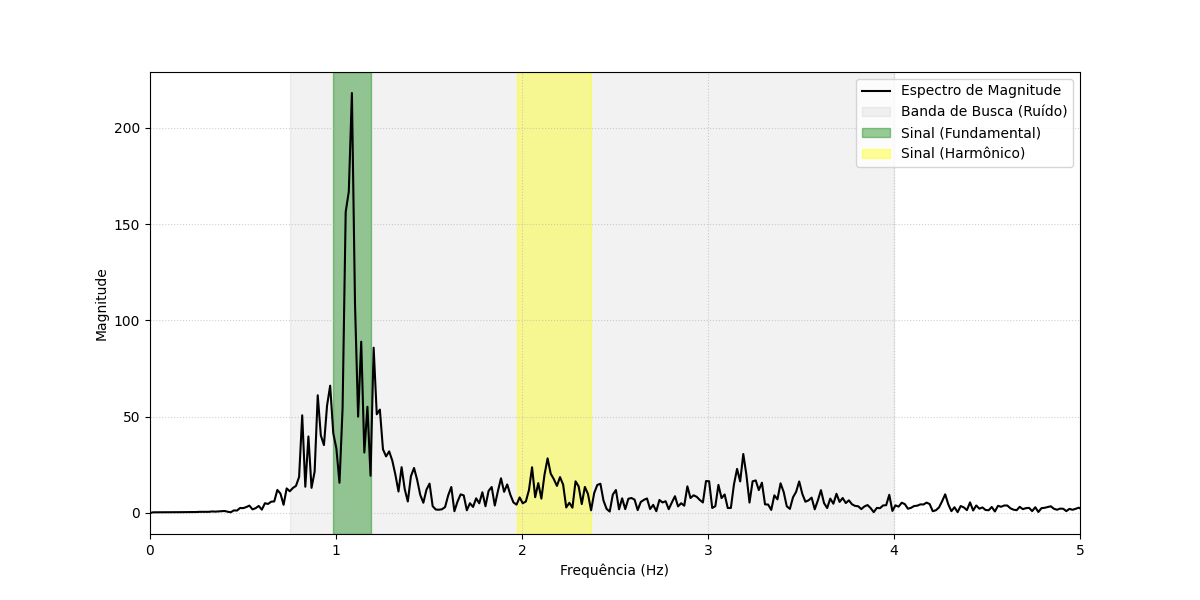
\includegraphics[width=1\linewidth]{imagens/snr_ex.png}
    \caption{Exemplo da definição da relação sinal-ruído}
    Fonte: autoria própria
    \label{fig:snr}
\end{figure}

Além disso, a fim de analisar as ondas de pulso de volume sanguíneo obtidas por cada método de rPPG, é realizada uma análise por correlação entre esse sinal e o sinal de fotopletismografia de referência, de modo que as duas ondas são sincronizadas por correlação cruzada e é calculado o índice de correlação de Pearson entre os sinais normalizados e sincronizados. Nesse caso, as amostras consideradas são os pontos do sinal de rPPG re-amostrado na frequência do sinal de referência. 
